\documentclass[12pt,a4paper]{article}
\usepackage[top=2.5cm,bottom=2.5cm,left=2.2cm,right=2.2cm]{geometry}
\usepackage{polski}
\usepackage[utf8]{inputenc}
%%\usepackage[OT4]{fontenc}
\usepackage{amsmath,amsfonts,amssymb,amsthm}
\usepackage{enumerate}
\usepackage{url}
\usepackage{multicol}
\usepackage{color}
\usepackage{graphicx} 
\usepackage{setspace}
\usepackage{float}
\usepackage{subfig}
\usepackage{listings}
\usepackage{pythonhighlight}
\usepackage{lipsum}
\usepackage{tabularx}
\usepackage{hyperref}

%\pagestyle{empty}
%WYMIARY STRONY
\topmargin -30mm
\oddsidemargin -1.7cm
\evensidemargin -1.7cm
\textwidth 180mm
\textheight 260mm
%\usepackage{psfrag}

\usepackage{amsmath}
\usepackage{amsfonts}

\usepackage{supertabular}
\usepackage{array}


\usepackage{tabularx}
\usepackage{hhline}

\newcommand{\myand}{i\ }
%\usepackage{showlabels}

\newcommand{\R}{I\!\!R} %symbol liczb rzeczywistych, dzia³a tylko w
                        %trybie matematycznym
\newtheorem{theorem}{Twierdzenie}[section] %nowe otoczenie do
                                           %sk³adania twierdzeñ

\usepackage{titlesec}
\titleformat*{\section}{\normalsize\bfseries}
\titleformat*{\subsection}{\footnotesize\bfseries}
\titleformat*{\subsubsection}{\normalsize}
\title{Uczenie ze wzmocnieniem}
\date{05.06.2018}
\author{Michał Bieroński, Łukasz Odwrot}

%ustawianie marginesów
\usepackage{geometry}
\newgeometry{tmargin=2.5cm, bmargin=2.5cm, lmargin=2.5cm, rmargin=2.5cm}


 
 
\begin{document}
\maketitle
\thispagestyle{empty}
\newpage
\tableofcontents
\setcounter{page}{1}
\newpage

\section{Opis algorytmów}
Zespoły klasyfikatorów wykorzystują wiele modeli decyzyjnych używających tego samego algorytmu. Zakłada się, że decyzja podjęta na podstawie głosu większości modeli jest prawidłowa. Do badań bazowym klasyfikatorem będzie \textit{Naive Bayes}. Głównymi metodami tworzenia zespołów klasyfikatorów są \textit{bagging} i \textit{boosting}. W przypadku pierwszej metody przykłady uczące losowane są ze zwracaniem, w drugim przypadku sytuacja wygląda podobnie, jednak szansa wylosowania każdego z przykładów odbywa się z różnym prawdopodobieństwem, zależnym od tego, jak dobrze radzą sobie wytrenowane już klasyfikatory.

\begin{figure}[H]
\centering
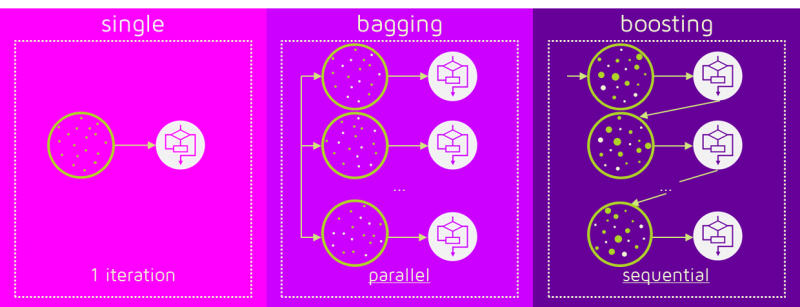
\includegraphics{choseWorks.png}
\caption{Losowanie przykładów uczących dla metod baging i boosting}
\end{figure}

Ponadto w przypadku metody \textit{bagging} głos każdego z klasyfikatorów liczony jest tak samo, w przypadku \textit{boostingu} każdy model ma przypisaną wagę głosu na podstawie jakości klasyfikacji. Niektóre modele mogą zostać odrzucone w przypadku zbyt niskiej jakości klasyfikacji (\textit{AdaBoost} wymaga 50\% skuteczności). 


\begin{figure}[H]
\centering
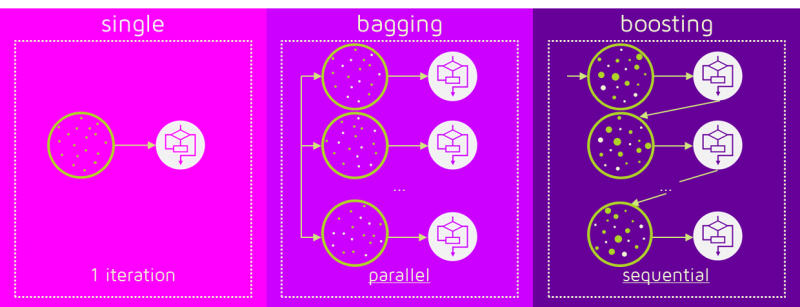
\includegraphics{choseWorks.png}
\caption{Przypisywanie wag modelom składowym}
\end{figure}
Zewnętrzne źródła podają, że użycie boostingu może w przypadku słabych klasyfikatorów dać bardzo dobre wyniki, a w przypadku boostingu prościej jest zapobiegać przeuczeniu poszczególnych modeli.\\
Oprócz tego zbadana zostanie metoda \textit{random forest}, która wykorzystuje wiele drzew decyzyjnych w celu podjęcia decyzji. Drzewa trenowane są zwykle w oparciu o \textit{bagging}.

\section{Opis badanych parametrów}
Dla każdej metody zbadany zostanie wpływ trzech parametrów na jakość klasyfikatorów. W przypadku dwóch pierwszych jako bazowy klasyfikator wykorzystany zostanie \textit{Naive Bayes}\\

Bagging:
\begin{itemize}
  \item n\_estimators - liczba klasyfikatorów,
  \item max\_samples  - odsetek przykładów dla każdego klasyfikatora jaki będzie brany z przykładów uczących,
  \item max\_features  - determinuje ilość cech jakie będą brane pod uwagę przy uczeniu poszczególnych klasyfikatorów
\end{itemize}

Boosting:
\begin{itemize}
  \item n\_estimators  - liczba klasyfikatorów,
  \item learning\_rate   - współczynnik obniżenia znaczenia każdego z klasyfikatorów,
  \item algorithm - algorytm używany przez algorytm ada-boost, w używanym pakiecie dostępne są ‘SAMME’ i ‘SAMME.R’.
\end{itemize}

Random Forest:
\begin{itemize}
  \item n\_estimators  - liczba klasyfikatorów,
  \item max\_features  - determinuje ilość cech jakie będą brane pod uwagę przy uczeniu poszczególnych klasyfikatorów
  \item max\_depth  - maksymalna liczba poziomów pojedynczego drzewa
\end{itemize}

\section{Badania metody bagging}
\begin{tabular}{ |p{3cm}||p{2cm}|p{2cm}|p{2cm}|p{2cm}| }
\hline
\multicolumn{5}{|c|}{wine}\\
\hline
n\_estimators & Accuracy & Precision & Recall & FScore \\
\hline
5.00 & 0.961 & 0.961 & 0.961 & 0.961\\
10.00 & 0.966 & 0.967 & 0.966 & 0.966\\
15.00 & 0.966 & 0.967 & 0.966 & 0.966\\
20.00 & 0.955 & 0.955 & 0.955 & 0.955\\
25.00 & 0.949 & 0.949 & 0.949 & 0.949\\
\hline
max\_samples & Accuracy & Precision & Recall & FScore \\
\hline
0.50 & 0.955 & 0.955 & 0.955 & 0.955\\
0.60 & 0.938 & 0.938 & 0.938 & 0.938\\
0.70 & 0.961 & 0.961 & 0.961 & 0.961\\
0.80 & 0.966 & 0.967 & 0.966 & 0.966\\
0.90 & 0.961 & 0.961 & 0.961 & 0.961\\
1.00 & 0.955 & 0.955 & 0.955 & 0.955\\
\hline
max\_features & Accuracy & Precision & Recall & FScore \\
\hline
0.50 & 0.910 & 0.910 & 0.910 & 0.910\\
0.60 & 0.955 & 0.955 & 0.955 & 0.955\\
0.70 & 0.944 & 0.944 & 0.944 & 0.944\\
0.80 & 0.966 & 0.966 & 0.966 & 0.966\\
0.90 & 0.944 & 0.944 & 0.944 & 0.944\\
1.00 & 0.961 & 0.961 & 0.961 & 0.961\\
\hline
\end{tabular}
\\
\begin{tabular}{ |p{3cm}||p{2cm}|p{2cm}|p{2cm}|p{2cm}| }
\hline
\multicolumn{5}{|c|}{glass}\\
\hline
n\_estimators & Accuracy & Precision & Recall & FScore \\
\hline
5.00 & 0.374 & 0.401 & 0.374 & 0.360\\
10.00 & 0.294 & 0.383 & 0.294 & 0.302\\
15.00 & 0.379 & 0.422 & 0.379 & 0.374\\
20.00 & 0.407 & 0.432 & 0.407 & 0.390\\
25.00 & 0.327 & 0.410 & 0.327 & 0.342\\
\hline
max\_samples & Accuracy & Precision & Recall & FScore \\
\hline
0.50 & 0.416 & 0.458 & 0.416 & 0.379\\
0.60 & 0.374 & 0.431 & 0.374 & 0.366\\
0.70 & 0.374 & 0.471 & 0.374 & 0.389\\
0.80 & 0.369 & 0.418 & 0.369 & 0.372\\
0.90 & 0.355 & 0.418 & 0.355 & 0.356\\
1.00 & 0.402 & 0.452 & 0.402 & 0.399\\
\hline
max\_features & Accuracy & Precision & Recall & FScore \\
\hline
0.50 & 0.379 & 0.440 & 0.379 & 0.374\\
0.60 & 0.402 & 0.420 & 0.402 & 0.391\\
0.70 & 0.397 & 0.423 & 0.397 & 0.389\\
0.80 & 0.355 & 0.380 & 0.355 & 0.349\\
0.90 & 0.341 & 0.411 & 0.341 & 0.353\\
1.00 & 0.425 & 0.449 & 0.425 & 0.409\\
\hline
\end{tabular}
\\
\begin{tabular}{ |p{3cm}||p{2cm}|p{2cm}|p{2cm}|p{2cm}| }
\hline
\multicolumn{5}{|c|}{diabetes}\\
\hline
n\_estimators & Accuracy & Precision & Recall & FScore \\
\hline
5.00 & 0.746 & 0.650 & 0.590 & 0.618\\
10.00 & 0.754 & 0.667 & 0.590 & 0.626\\
15.00 & 0.758 & 0.669 & 0.604 & 0.635\\
20.00 & 0.754 & 0.664 & 0.597 & 0.629\\
25.00 & 0.753 & 0.664 & 0.590 & 0.625\\
\hline
max\_samples & Accuracy & Precision & Recall & FScore \\
\hline
0.50 & 0.754 & 0.664 & 0.597 & 0.629\\
0.60 & 0.759 & 0.671 & 0.608 & 0.638\\
0.70 & 0.755 & 0.668 & 0.593 & 0.628\\
0.80 & 0.745 & 0.650 & 0.582 & 0.614\\
0.90 & 0.754 & 0.664 & 0.597 & 0.629\\
1.00 & 0.749 & 0.653 & 0.597 & 0.624\\
\hline
max\_features & Accuracy & Precision & Recall & FScore \\
\hline
0.50 & 0.755 & 0.700 & 0.522 & 0.598\\
0.60 & 0.743 & 0.698 & 0.466 & 0.559\\
0.70 & 0.749 & 0.673 & 0.545 & 0.602\\
0.80 & 0.757 & 0.669 & 0.597 & 0.631\\
0.90 & 0.753 & 0.662 & 0.593 & 0.626\\
1.00 & 0.753 & 0.664 & 0.590 & 0.625\\
\hline
\end{tabular}

\section{Badania metody ADA-Boosting}
\begin{tabular}{ |p{3cm}||p{2cm}|p{2cm}|p{2cm}|p{2cm}| }
\hline
\multicolumn{5}{|c|}{wine}\\
\hline
n\_estimators & Accuracy & Precision & Recall & FScore \\
\hline
5.00 & 0.803 & 0.805 & 0.803 & 0.802\\
10.00 & 0.815 & 0.825 & 0.815 & 0.816\\
20.00 & 0.921 & 0.925 & 0.921 & 0.921\\
30.00 & 0.899 & 0.903 & 0.899 & 0.899\\
40.00 & 0.949 & 0.951 & 0.949 & 0.950\\
50.00 & 0.916 & 0.922 & 0.916 & 0.915\\
60.00 & 0.938 & 0.939 & 0.938 & 0.938\\
70.00 & 0.966 & 0.967 & 0.966 & 0.966\\
\hline
learning\_rate & Accuracy & Precision & Recall & FScore \\
\hline
0.80 & 0.972 & 0.972 & 0.972 & 0.972\\
0.85 & 0.921 & 0.931 & 0.921 & 0.922\\
0.90 & 0.927 & 0.929 & 0.927 & 0.927\\
0.95 & 0.961 & 0.961 & 0.961 & 0.961\\
1.00 & 0.916 & 0.922 & 0.916 & 0.915\\
\hline
algorithm & Accuracy & Precision & Recall & FScore \\
\hline
SAMME & 0.966 & 0.966 & 0.966 & 0.966\\
SAMME.R & 0.916 & 0.922 & 0.916 & 0.915\\
\hline
\end{tabular}

.\\
\begin{tabular}{ |p{3cm}||p{2cm}|p{2cm}|p{2cm}|p{2cm}| }
\hline
\multicolumn{5}{|c|}{glass}\\
\hline
n\_estimators & Accuracy & Precision & Recall & FScore \\
\hline
5.00 & 0.425 & 0.442 & 0.425 & 0.429\\
10.00 & 0.421 & 0.464 & 0.421 & 0.420\\
20.00 & 0.481 & 0.529 & 0.481 & 0.492\\
30.00 & 0.528 & 0.575 & 0.528 & 0.535\\
40.00 & 0.598 & 0.631 & 0.598 & 0.599\\
50.00 & 0.584 & 0.627 & 0.584 & 0.575\\
60.00 & 0.551 & 0.587 & 0.551 & 0.537\\
70.00 & 0.593 & 0.590 & 0.593 & 0.573\\
\hline
learning\_rate & Accuracy & Precision & Recall & FScore \\
\hline
0.80 & 0.565 & 0.626 & 0.565 & 0.550\\
0.85 & 0.519 & 0.534 & 0.519 & 0.482\\
0.90 & 0.523 & 0.543 & 0.523 & 0.509\\
0.95 & 0.547 & 0.563 & 0.547 & 0.539\\
1.00 & 0.584 & 0.627 & 0.584 & 0.575\\
\hline
algorithm & Accuracy & Precision & Recall & FScore \\
\hline
SAMME & 0.379 & 0.442 & 0.379 & 0.395\\
SAMME.R & 0.584 & 0.627 & 0.584 & 0.575\\
\hline
\end{tabular}
\\

\begin{tabular}{ |p{3cm}||p{2cm}|p{2cm}|p{2cm}|p{2cm}| }
\hline
\multicolumn{5}{|c|}{diabetes}\\
\hline
n\_estimators & Accuracy & Precision & Recall & FScore \\
\hline
5.00 & 0.645 & 0.472 & 0.157 & 0.235\\
10.00 & 0.503 & 0.397 & 0.821 & 0.535\\
20.00 & 0.484 & 0.373 & 0.698 & 0.486\\
30.00 & 0.556 & 0.368 & 0.381 & 0.374\\
40.00 & 0.559 & 0.391 & 0.478 & 0.430\\
50.00 & 0.533 & 0.390 & 0.604 & 0.474\\
60.00 & 0.591 & 0.421 & 0.455 & 0.437\\
70.00 & 0.589 & 0.430 & 0.549 & 0.482\\
\hline
learning\_rate & Accuracy & Precision & Recall & FScore \\
\hline
0.80 & 0.546 & 0.414 & 0.724 & 0.526\\
0.85 & 0.518 & 0.377 & 0.582 & 0.457\\
0.90 & 0.531 & 0.372 & 0.496 & 0.425\\
0.95 & 0.617 & 0.453 & 0.463 & 0.458\\
1.00 & 0.533 & 0.390 & 0.604 & 0.474\\
\hline
algorithm & Accuracy & Precision & Recall & FScore \\
\hline
SAMME & 0.760 & 0.688 & 0.575 & 0.626\\
SAMME.R & 0.533 & 0.390 & 0.604 & 0.474\\
\hline
\end{tabular}
\\
\section{Badania metody Random Forest}

\begin{tabular}{ |p{3cm}||p{2cm}|p{2cm}|p{2cm}|p{2cm}| }
\hline
\multicolumn{5}{|c|}{wine}\\
\hline
n\_estimators & Accuracy & Precision & Recall & FScore \\
\hline
5.00 & 0.955 & 0.956 & 0.955 & 0.955\\
10.00 & 0.978 & 0.978 & 0.978 & 0.978\\
15.00 & 0.949 & 0.950 & 0.949 & 0.949\\
20.00 & 0.972 & 0.974 & 0.972 & 0.972\\
25.00 & 0.955 & 0.956 & 0.955 & 0.955\\
\hline
max\_features & Accuracy & Precision & Recall & FScore \\
\hline
0.50 & 0.978 & 0.978 & 0.978 & 0.978\\
0.60 & 0.955 & 0.955 & 0.955 & 0.955\\
0.70 & 0.944 & 0.944 & 0.944 & 0.943\\
0.80 & 0.921 & 0.924 & 0.921 & 0.921\\
0.90 & 0.933 & 0.933 & 0.933 & 0.933\\
1.00 & 0.944 & 0.944 & 0.944 & 0.944\\
\hline
max\_depth & Accuracy & Precision & Recall & FScore \\
\hline
3.00 & 0.944 & 0.947 & 0.944 & 0.944\\
4.00 & 0.961 & 0.962 & 0.961 & 0.960\\
5.00 & 0.944 & 0.944 & 0.944 & 0.944\\
6.00 & 0.961 & 0.961 & 0.961 & 0.960\\
7.00 & 0.933 & 0.934 & 0.933 & 0.933\\
8.00 & 0.966 & 0.966 & 0.966 & 0.966\\
\hline
\end{tabular}
\\
\\.
\begin{tabular}{ |p{3cm}||p{2cm}|p{2cm}|p{2cm}|p{2cm}| }
\hline
\multicolumn{5}{|c|}{glass}\\
\hline
n\_estimators & Accuracy & Precision & Recall & FScore \\
\hline
5.00 & 0.650 & 0.648 & 0.650 & 0.647\\
10.00 & 0.678 & 0.668 & 0.678 & 0.667\\
15.00 & 0.654 & 0.654 & 0.654 & 0.649\\
20.00 & 0.664 & 0.666 & 0.664 & 0.653\\
25.00 & 0.678 & 0.675 & 0.678 & 0.671\\
\hline
max\_features & Accuracy & Precision & Recall & FScore \\
\hline
0.50 & 0.664 & 0.657 & 0.664 & 0.657\\
0.60 & 0.682 & 0.690 & 0.682 & 0.681\\
0.70 & 0.636 & 0.634 & 0.636 & 0.631\\
0.80 & 0.650 & 0.649 & 0.650 & 0.643\\
0.90 & 0.668 & 0.671 & 0.668 & 0.662\\
1.00 & 0.626 & 0.619 & 0.626 & 0.612\\
\hline
max\_depth & Accuracy & Precision & Recall & FScore \\
\hline
3.00 & 0.612 & 0.568 & 0.612 & 0.582\\
4.00 & 0.678 & 0.706 & 0.678 & 0.657\\
5.00 & 0.654 & 0.653 & 0.654 & 0.644\\
6.00 & 0.673 & 0.684 & 0.673 & 0.660\\
7.00 & 0.640 & 0.644 & 0.640 & 0.630\\
8.00 & 0.682 & 0.685 & 0.682 & 0.679\\
\hline
\end{tabular}
\\
\\.
\begin{tabular}{ |p{3cm}||p{2cm}|p{2cm}|p{2cm}|p{2cm}| }
\hline
\multicolumn{5}{|c|}{diabetes}\\
\hline
n\_estimators & Accuracy & Precision & Recall & FScore \\
\hline
5.00 & 0.732 & 0.624 & 0.582 & 0.602\\
10.00 & 0.738 & 0.652 & 0.537 & 0.589\\
15.00 & 0.759 & 0.675 & 0.597 & 0.634\\
20.00 & 0.746 & 0.665 & 0.549 & 0.601\\
25.00 & 0.755 & 0.675 & 0.575 & 0.621\\
\hline
max\_features & Accuracy & Precision & Recall & FScore \\
\hline
0.50 & 0.737 & 0.657 & 0.515 & 0.577\\
0.60 & 0.758 & 0.703 & 0.530 & 0.604\\
0.70 & 0.754 & 0.689 & 0.537 & 0.604\\
0.80 & 0.740 & 0.656 & 0.534 & 0.588\\
0.90 & 0.754 & 0.682 & 0.552 & 0.610\\
1.00 & 0.754 & 0.685 & 0.545 & 0.607\\
\hline
max\_depth & Accuracy & Precision & Recall & FScore \\
\hline
3.00 & 0.757 & 0.731 & 0.478 & 0.578\\
4.00 & 0.755 & 0.696 & 0.530 & 0.602\\
5.00 & 0.760 & 0.696 & 0.556 & 0.618\\
6.00 & 0.753 & 0.682 & 0.545 & 0.606\\
7.00 & 0.757 & 0.685 & 0.560 & 0.616\\
8.00 & 0.747 & 0.661 & 0.567 & 0.610\\
\hline
\end{tabular}
\\

\section{Optymalne wartości parametrów dla zbiorów i porównania}
Dla każdego zestawu danych i każdej metody wybrane zostały wyznaczone optymalne wartości parametrów. \\Dla metody bagging wartości parametrów kolejno: n\_estimators, max\_samples, max\_features

\begin{enumerate}
  \item wine: 15, 0.8, 0.8
  \item glass: 20, 1.0, 1.0
  \item diabetes:15, 0.6, 0.8
\end{enumerate}

Dla metody bagging wartości parametrów kolejno: n\_estimators, learning\_rate, algorithm

\begin{enumerate}
  \item wine: 70, 0.8, 'SAMME'
  \item glass: 40, 1.0, 'SAMME.R'
  \item diabetes: 10, 0.8, 'SAMME'
\end{enumerate}

Dla metody random forest wartości parametrów kolejno: n\_estimators, max\_features, max\_depth

\begin{enumerate}
  \item wine: 10, 0.5, 8
  \item glass: 25, 0.6, 8
  \item diabetes: 15, 0.9, 5
\end{enumerate}

Rezultaty zestawiono z wynikami z poprzednich laboratoriów.

\begin{tabular}{ |p{3cm}||p{2cm}|p{2cm}|p{2cm}|p{2cm}| }
\hline
Metoda & Wine & Diabetes & Glass \\
\hline
C4.5 & 0.932 & 0.816 & 0.691\\
NaiveBayes & 0.957 & 0.748 & 0.646\\
Knn & 0.972 & 0.690 & 0.608\\
Baging & 0.966 & 0.643 & 0.671\\
Boosting & 0.922 & 0.6 & 0.291\\
Random Fores & 0.949 & 0.631 & 0.689\\
\hline
\end{tabular}

\begin{figure}[H]
\centering
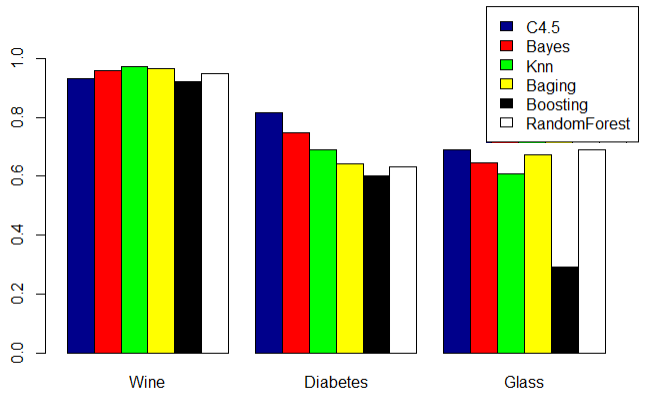
\includegraphics{versusGraphic.PNG}
\caption{Porównanie rezultatów różnych metod klasyfikacji}
\end{figure}

\section{Wnioski}
Zastosowane metody na relatywnie słabym, niesparametryzowanym modelu dały porównywalne rezultaty do badanych na poprzednich zajęciach. Optymalizacja klasyfikatora bazowego, albo jego zmiana mogłyby znaczącą wpłynąć na poprawę wyników.

\end{document}




